
 \chapter{Apartados del CUERPO DEL DOCUMENTO}

El llamado ``cuerpo del documento'' es el grupo de apartados donde se describe como  se ha desarrollado el trabajo. En el dominio de la Informática, un TFG debe mantener un equilibrio entre la componente de investigación y la componente puramente técnica asociada con el proyecto de desarrollo de software. Un projecto software conlleva la elaboración de una serie de memorias, cada una recopilando lo hecho a distintos niveles, ver figura \ref{fig:report}. Sin embargo la memoria de un TFG es de carácter académico y ademas de artefactos, presupuestos y modelos debe incluir determinadas cuestiones que muestren como se han desarrollado las ideas propias. El punto de partida es la estructura típica de un articulo que se muestra en la figura \ref{fig:articulo}.


\begin{figure}

	\begin{center}
		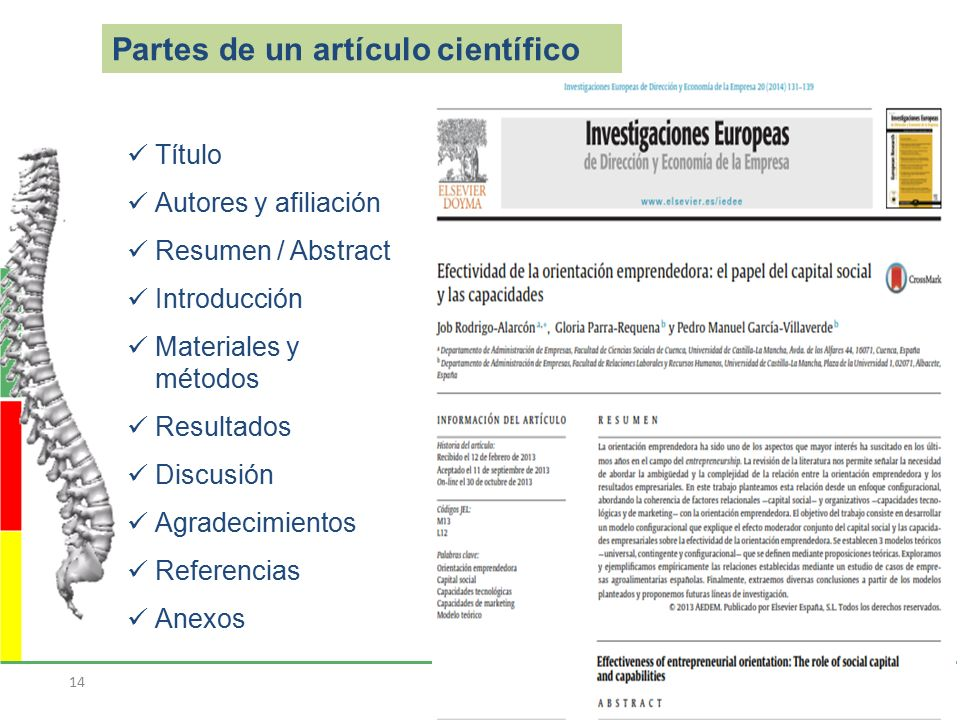
\includegraphics[scale = 0.45]{Figuras/articulo.jpg}
	\end{center}
	\caption{Estructura clásica de un articulo de investigación}
	\label{fig:articulo}
\end{figure}


\begin{figure}  
 	\begin{center}
        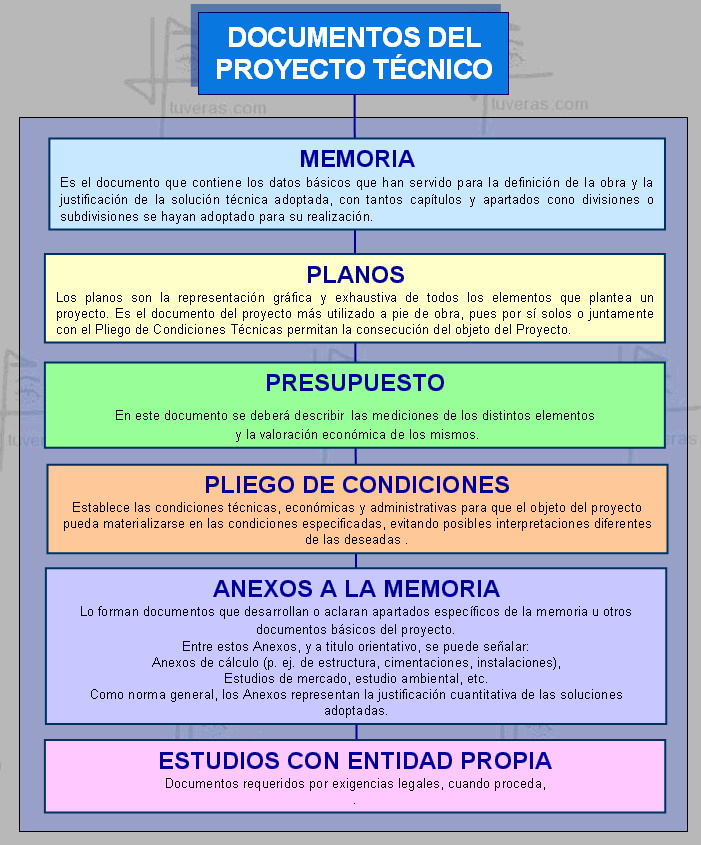
\includegraphics[scale = 0.45]{Figuras/documentos.jpg}
        	\end{center}
        \caption{Estructura de documentos de un proyecto técnico}
    \label{fig:report}
\end{figure}


La propuesta de estructura se define a continuación indicando que se incluiría en cada apartado. Lo importante en este caso es \textsc{que hay que incluir} la estructura del TFG final de cada alumno puede ser diferente, uniendo o separando los contenidos que se detallan a continuación. 

\paragraph{Objetivos o cuestiones de investigación}

se establecerá el objetivo general y los específicos, es decir, cuestiones que serán respondidas con el trabajo que se va a realizar. No es
imprescindible elaborar un apartado específico denominado OBJETIVOS, pues éstos puede quedar reflejados al final de la
introducción

\paragraph{Planificación temporal} 
Se debe incluir una referencia a como se han distribuido las tareas a lo largo del tiempo empleado en el TFG. Esta cuestión deriva de los proyectos técnicos de disciplinas de ingeniería. Puede representarse en forma de tabla o gráfico \ref{fig:plan} y puede aparecer dentro del apartado de metodología.



\begin{figure} 
\begin{ganttchart}[
hgrid,
vgrid={*6{draw=none},dotted},
x unit=0.5mm,
y unit title =0.6cm,
y unit  chart=1cm,
canvas/.style={draw=none},
%title/.append style={fill=black!10, rounded corners=1mm},
title/.append style={ rounded corners=0.5mm},
time slot format=isodate,
time slot format/base century=2000,
time slot unit= day,
time slot format/start date=2020-11-25,
bar height=0.5,
 bar label node/.append style={left=0.01cm, align=left, text width=8em},
 bar label text={$\star$#1},
 bar label font=\sffamily\footnotesize,
 group label node/.append style={left=0.01cm, align=left, text width=8em},
  group peaks width={3},
   group label font=\bfseries\footnotesize,
milestone label font=\scshape\sffamily\footnotesize,
  milestone inline label node/.append style={left=5mm},
  milestone right shift=2,
    milestone left shift=-2,
 milestone/.append style={fill=black!40}
]{2020-11-24}{2021-06-30}
\gantttitlecalendar[y unit title=0.7cm, title height=0.6]{year, month=shortname ,week} \\

\ganttgroup[ bar height=.1]{Selección área}{2020-11-24}{2020-11-30} \\
\ganttbar[name=b2]{Envío de Correos de contacto}{2020-11-24}{2020-11-26}\\
\ganttbar[name=b2]{Realizar Entrevistas}{2020-11-27}{2020-11-30}\\
\ganttmilestone{Área y tutor definido}{2020-11-30} \\ %\ganttnewline
\ganttgroup[bar height=.1]{Estudio preliminar}{2020-12-01}{2020-12-22}\\
\ganttlinkedbar{Task 2}{2020-12-01}{2020-12-22} \\
\ganttbar{Final Task}{2020-12-01}{2020-12-22}\\
\ganttbar{Task 2}{2020-12-01}{2020-12-22}
%\ganttlink{elem2}{elem3}
%\ganttlink{elem3}{elem4}
\end{ganttchart}
        \caption{Planificación del proyecto sobre latex}
    \label{fig:planb}
\end{figure}


\begin{figure}  
 	\begin{center}
        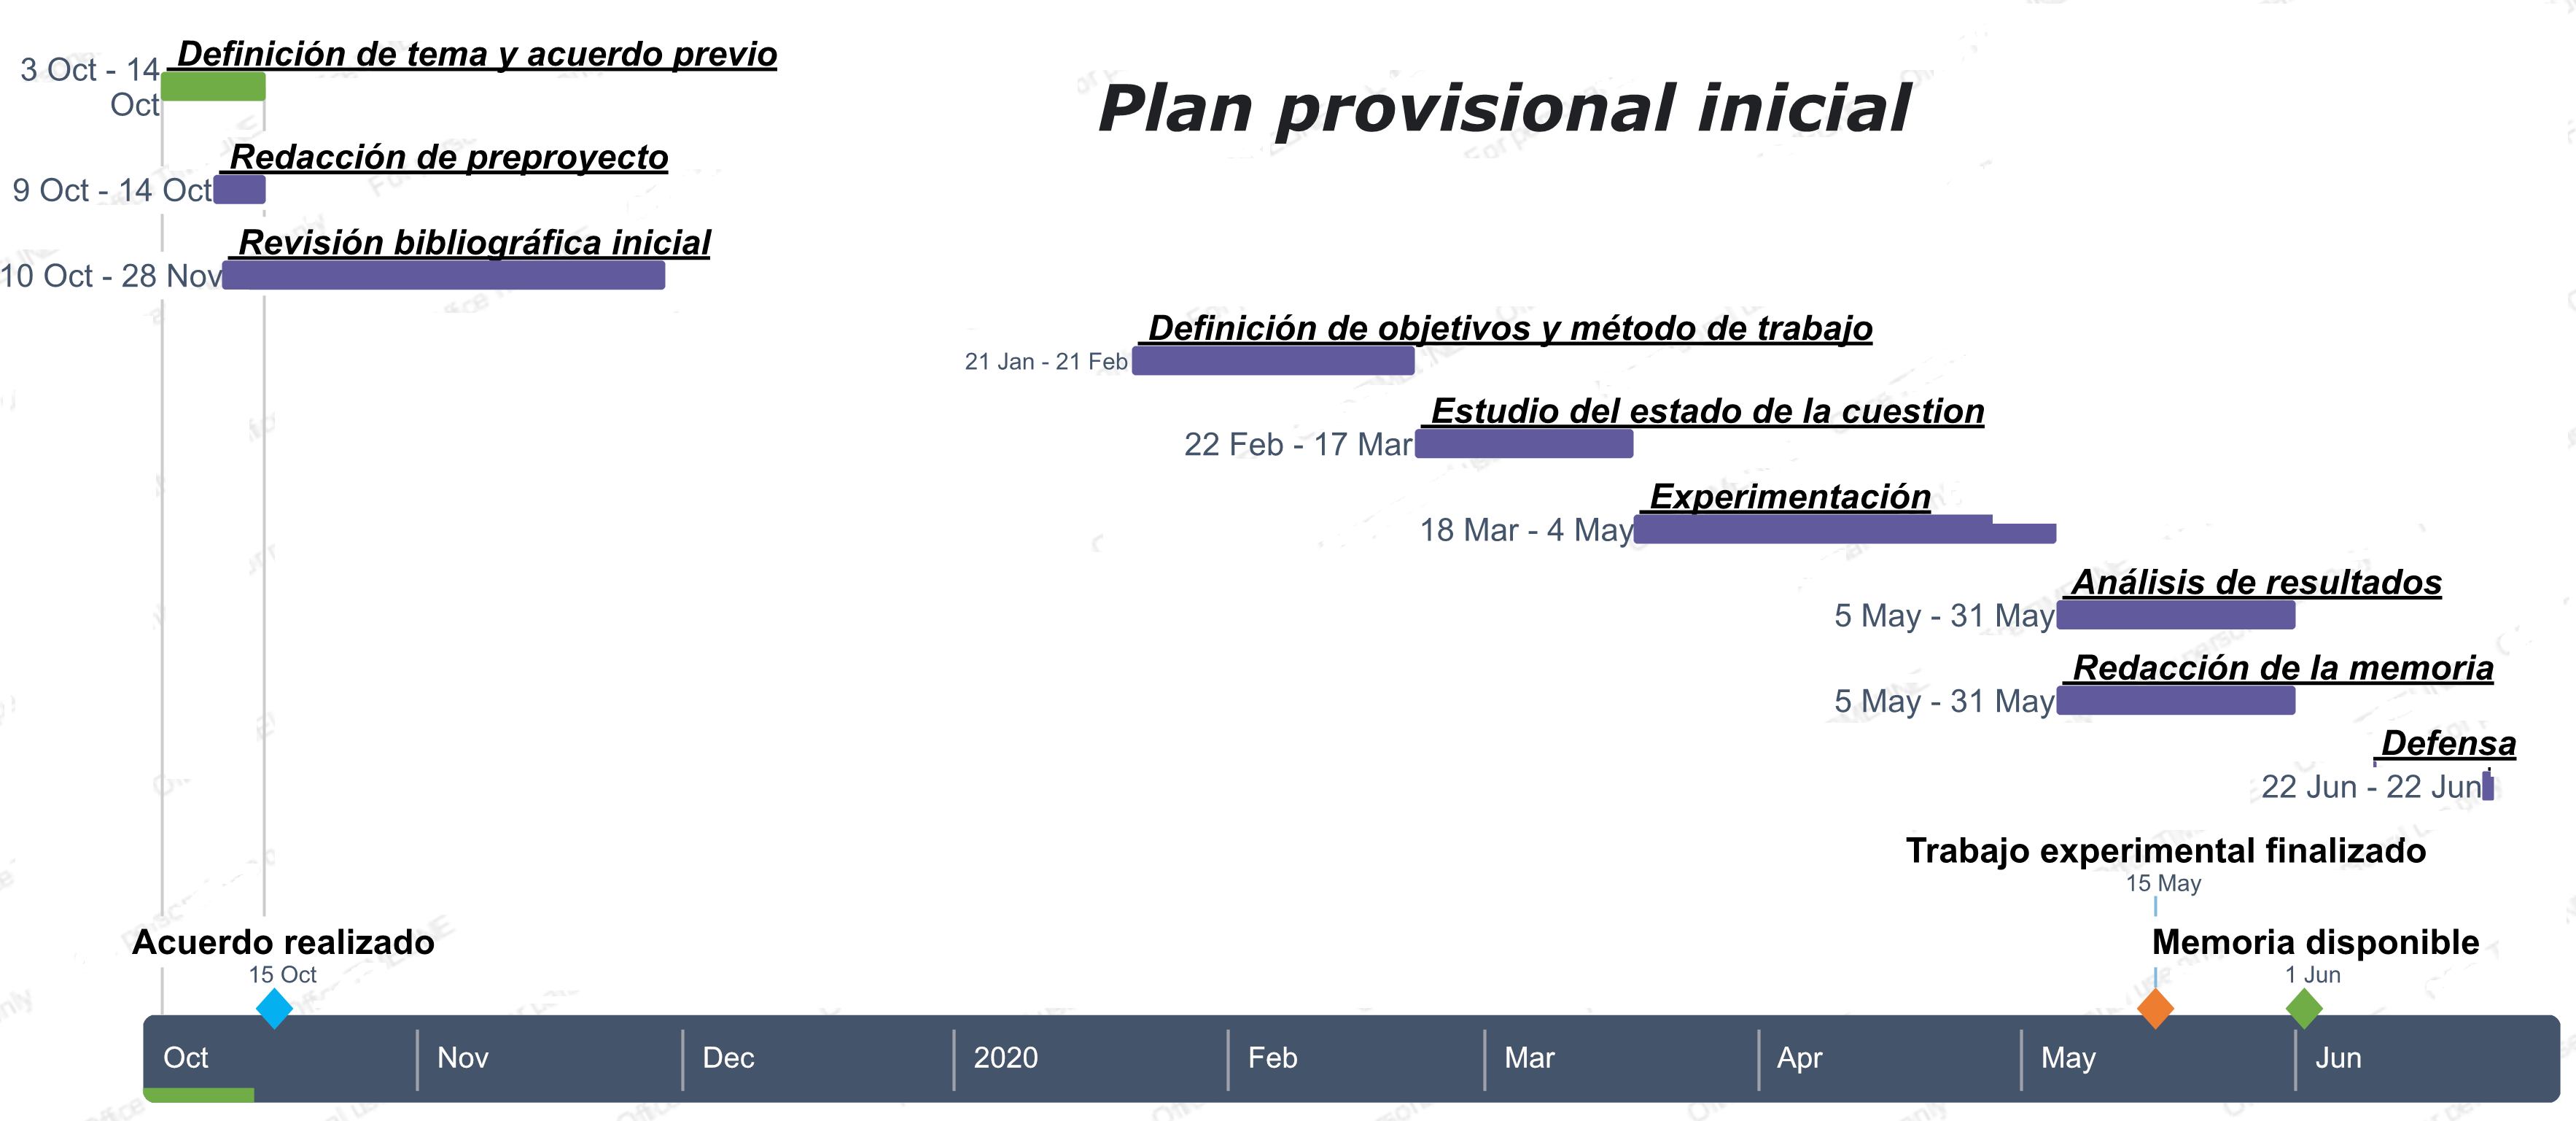
\includegraphics[width=0.8\textwidth]{Figuras/plandef.png}
        	\end{center}
        \caption{Planificación del proyecto}
    \label{fig:plan}
\end{figure}

\paragraph{Contextualización o estado del arte}

Se hará mención a los elementos conceptuales que  sirven  de  base  para  la  investigación,  estudios  previos  relacionados  con  el problema planteado, etc. En este apartado es importante hacer un estudio de los trabajos previos o revisión bibliográfica \cite{kitchenham2009systematic,kitchenham_2013}. Si como es habitual se tiene  que utilizar una o varias herramientas software es en este apartado donde se recogen las alternativas consideradas y cual de ellas ha sido elegida  y porqué.

\paragraph{Metodología}
¿Qué procedimiento se ha seguido para alcanzar los objetivos
planteados? Se  indicará  el  tipo  o  tipos  de  investigación,  las  técnicas  y  los procedimientos  que  serán  utilizados  para  llevarla  a  cabo;  se  identificará la población  y  el  tamaño  de  la  muestra  así  como  las técnicas  e  instrumentos  de recolección de datos, si te trata de un trabajo empírico, la metodología de desarrollo de software seleccionada. O cualquier otra información sobre el proceso seguido. La planificación y objetivos también pueden estar en este apartado

 
\paragraph{Resultados}
Incluirá  los  resultados  de  la  investigación  o  trabajo,  así como el análisis y la discusión de los mismos, aunque algunos tutores prefieren dos apartados separados. En el caso de tratarse de un desarrollo de software en este apartado se incluirá la descripción del producto resultante y los modelos o artefactos softtware necesarios para su descripción. Pero el manual o tutorial detallado  y los modelos completos deberían llevarse a los anexos.


La discusión conlleva revisar que aporta el trabajo realizado y se  han conseguido los objetivos planteados inicialmente. Caso de tener una evaluación por parte de los clientes potenciales también aparecerá en este apartado.


 \chapter{Apartado BIBLIOGRAFIA}
 Este apartado es de vital importancia para tener éxito en la consecución del trabajo fin de grado. Los tribunales suelen prestar gran atención a este apartado, probablemente por su formación académica. 
 
 Es todo un mundo el de los estilos bibliográficos y la realización de las citas, se puede encontrar un tutorial en:  \url{http://ci2.ual.es/comunicar-la-informacion/citas-y-referencias-bibliograficas/}. No obstante en las siguientes secciones se indicarán las cuestiones básicas para iniciarse en el tema pero restringuiendose a la utilización de la presente plantilla. La gran ventaja de latex es que cada elemento en las referencias   \lstinline[language=enparrafo]!\bibitem! es considerado como un elemento de una base de datos, de forma que es el compilador el que reordena o coloca la cita de acuerdo con el estilo definido.

 \section{Como citar}
A lo largo del texto de la memoria se incluirán citas a trabajos de otros autores. La inclusión de la cita tiene que ser justo después del texto donde se propone algo relativo al trabajo citado. Para citar, como para todo el \LaTeX{} existen numerosos paquetes, los dos mas conocidos son  biblatex y   natbib . 

Además dada forma de citar y de incorporar items en el apartado referencias lleva asociado un estilo de bibliografía    \lstinline[language=enparrafo]!\bibliographystyle{XXX}!, que aun abre mucho mas el abanico de opciones. 

Es recomendable consultar las ayudas de los paquetes \url{https://www.overleaf.com/learn/latex/Biblatex_bibliography_styles} y \url{https://www.overleaf.com/learn/latex/Bibliography_management_with_natbib}.

Lo habitual es utilizar la orden      \lstinline[language=enparrafo]!\cite{xxx}!, o   \lstinline[language=enparrafo]!\citep(xxx)!  en la ubicación en el texto donde se quiere colocar la cita, el compilador se encargá de procesarla según el estilo.

 \section {Apartado referencias}
  Existen dos formas de incorporar las referencias, directamente en el entorno   \lstinline[language=enparrafo]!\begin{bibliography}! y utilizando las ordenes del lenguaje o bien utilizando un archivo .bib para guardar esas referencias. Se generará un auxiliar .bbl que automáticamente se incorpora en el documento.
  
  Este archivo auxiliar es el que tiene directamente las ordenes del lenguaje.
  
 \begin{verbatim}
  
\begin{thebibliography}{3}

\bibitem{SWEBOK2014}
P.~Bourque and R.~E. Fairley, Eds., \emph{{SWEBOK}: Guide to the Software
  Engineering Body of Knowledge}, version 3.0~ed.\hskip 1em plus 0.5em minus
  0.4em\relax Los Alamitos, CA: IEEE Computer Society, 2014.

\bibitem{kitchenham_2013}
B.~Kitchenham and P.~Brereton, ``A systematic review of systematic review
  process research in software engineering,'' \emph{Information and Software
  Technology}, vol.~55, no.~12, pp. 2049 -- 2075, 2013.

\bibitem{basili1992}
V.~R. Basili, ``Software modeling and measurement: the goal/question/metric
  paradigm. cs-tr-2956, umiacs-tr-92-96,'' University of Maryland, Tech. Rep.,
  1992.
\end{thebibliography}

  \end{verbatim}
 
 
 
 \section{Archivos .bib}
 
 BibTeX, y natbib por extensión, usan un archivo externo en texto plano como base de datos de referencias bibliográficas para generar las bibliografías y sus referencias en documentos con distintos formatos de artículos, libros, tesis, presentaciones, etc. Los nombres de archivos de referencias bibliográficas de BibTeX usualmente terminan o usan la extensión .bib. Los ítems bibliográficos incluidos en un .bib están separados por tipos.
 
 \begin{verbatim}
@inbook{Berander2005,
        address = {Berlin, Heidelberg},
        author = {Berander, Patrik and Andrews, Anneliese},
        booktitle = {Engineering and Managing Software Requirements},
        pages = {69--94},
        publisher = {Springer Berlin Heidelberg},
        title = {{Requirements Prioritization}},
        doi= {https://doi.org/10.1007/3-540-28244-0{\_}4},
        year = {2005}
} 
 \end{verbatim}
 
 Los tipos que son reconocidos por virtualmente todos los estilos de BibTeX se muestran en el anexo \ref{sec:bib}. Pero igual que antes es recomendable recurrir a tutoriales o recursos donde se describan con detalle. Además se recomienda la utilización de algún gestor de referencias bibliográficas tipo Mendeley. \url{https://www.mendeley.com/}
 
 \flimage{Captura}{Hola captura}